\section{실험 과정}

\subsection{준비}
$\rm{CsPbBr_3}$ 용액은 실온 1기압 상태에서 제작되었다. $\rm{CsPbBr_3}$의 용액을 만들기 위해서 $\rm{CsBr}$과 $\rm{PbBr_2}$를 1:1의 몰 비율로 $\rm{CsBr}$ 0.638g과 $\rm{PbBr_2}$ 1.101 g을 섞었으며 용매인 Dimethyl Sulfoxide (DMSO) 6ml에 섞었다. 용매와 용질을 균일하게 섞기 위해서 50ml들이 통에 담은 후 뚜껑 부분을 파라필름으로 밀봉하고, 통을 물이 담긴 비커에 담은 후 초음파를 이용한 Sonication을 3분간 진행하였다. 
\begin{figure}[h!]
	\begin{center}
		\begin{tabular}{ccc}
			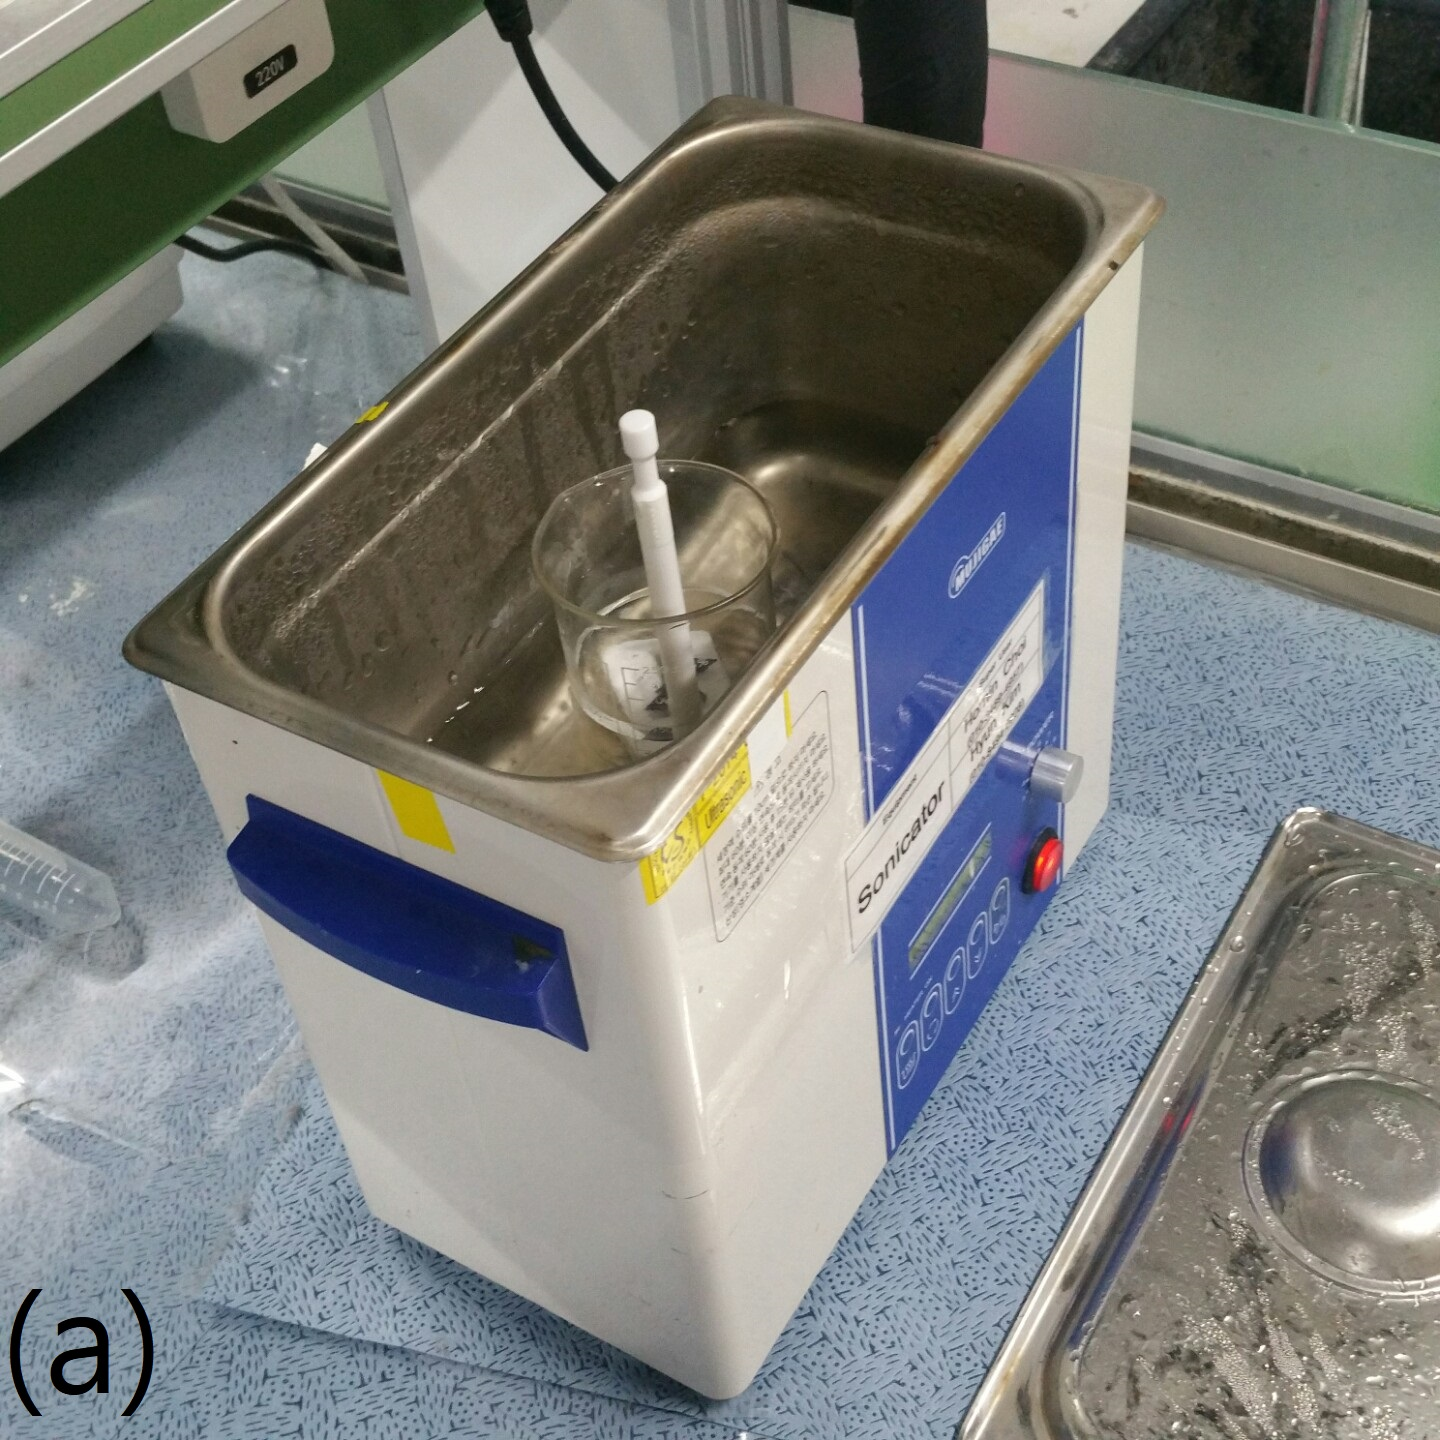
\includegraphics[width=4cm]{sonic} &   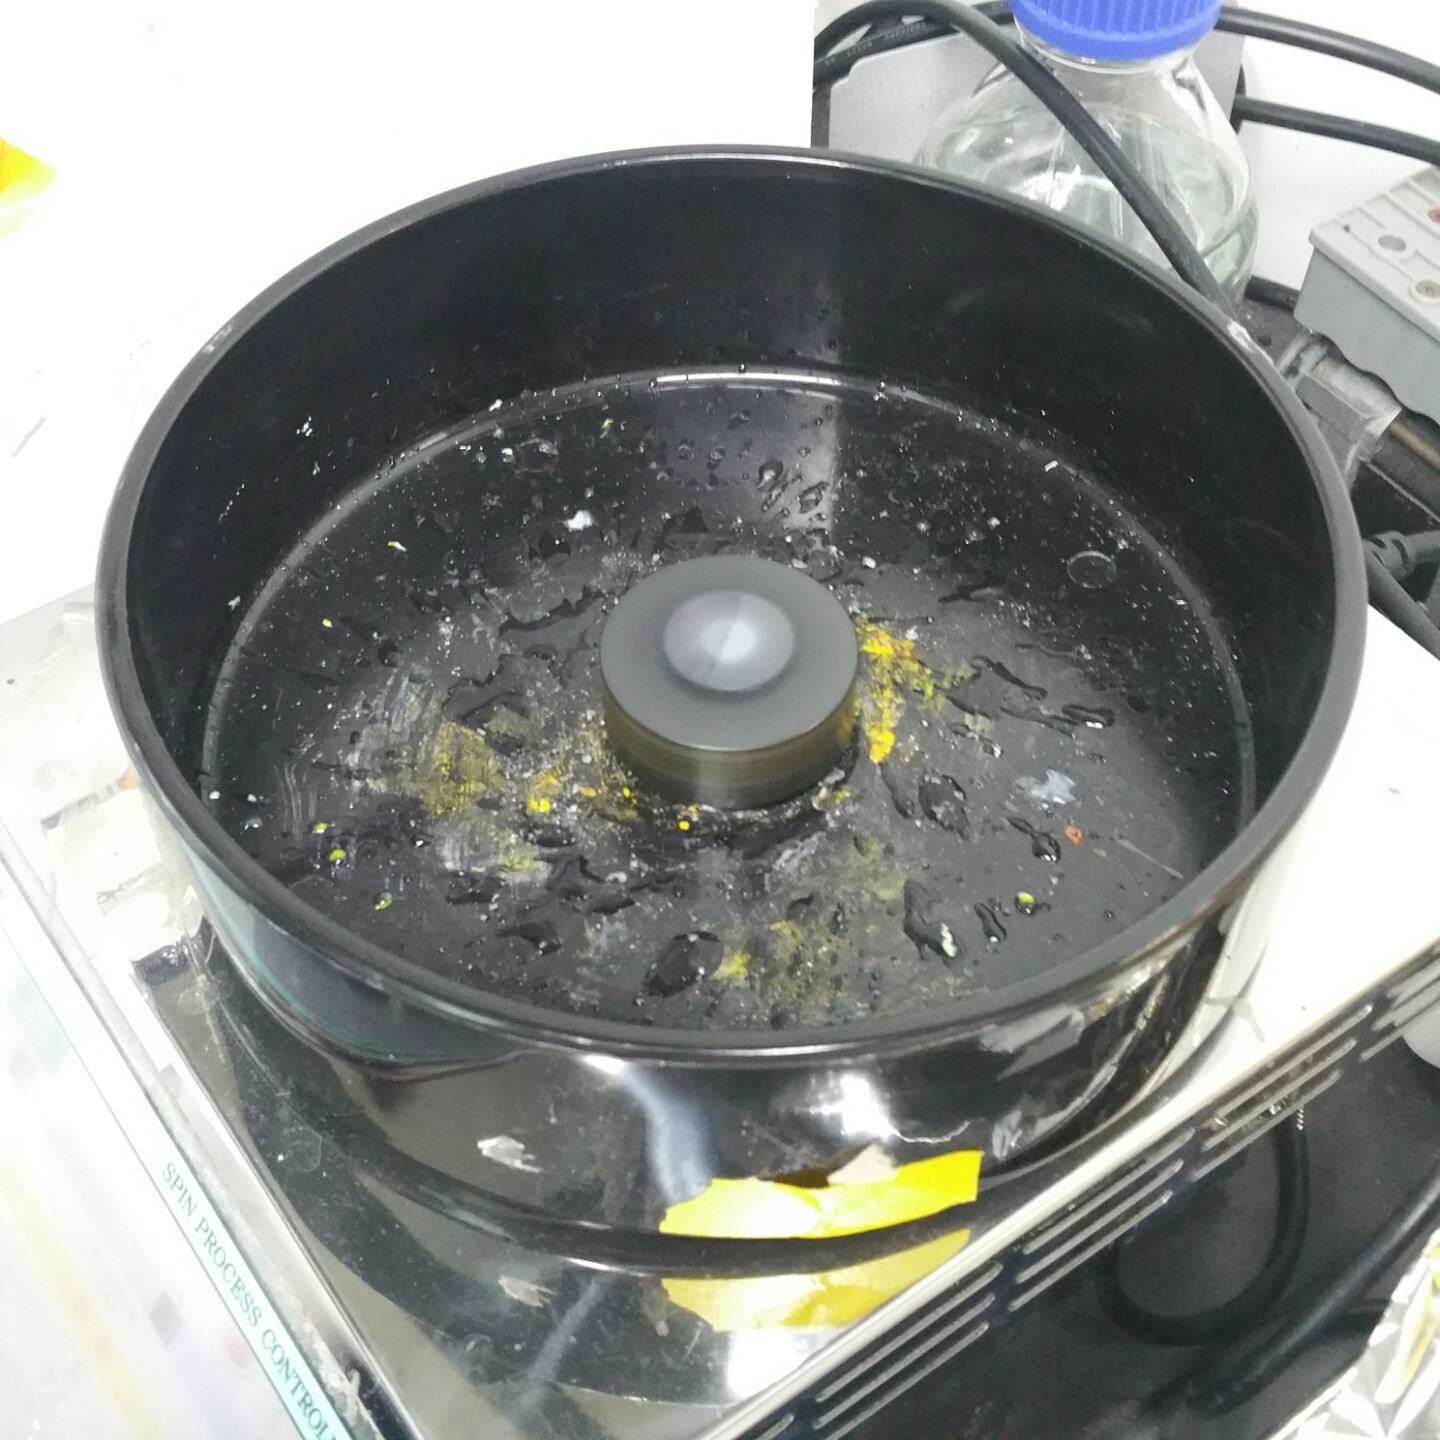
\includegraphics[width=4cm]{spin_coater} &
			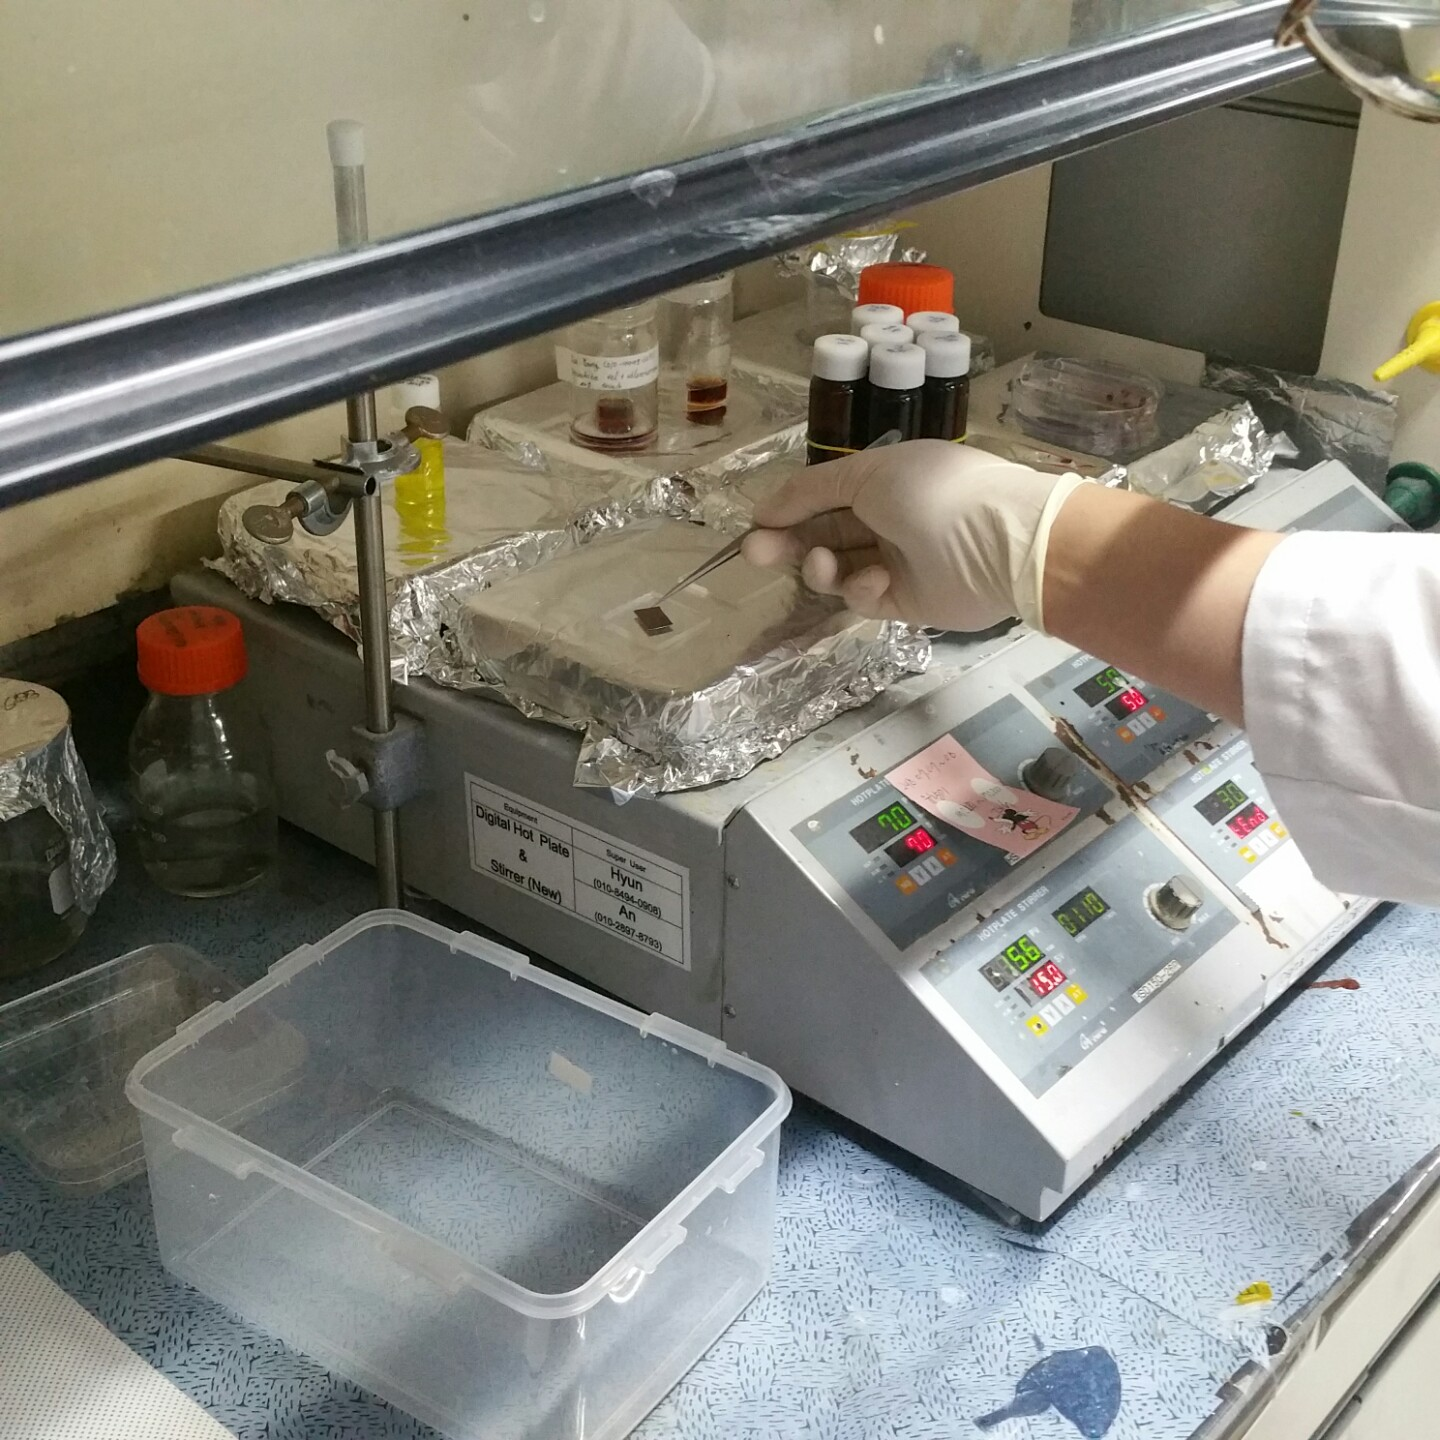
\includegraphics[width=4cm]{pdms_stamping}
		\end{tabular}
		\caption{Pictures show the sonication process, spin-coating process, and PDMS stamping process, respectively.}	
		\label{fig:FIR221}
	\end{center}
\end{figure}
또, Sonication으로 세척한 Silicon wafer 위에 O2 plasma를 이용하여 코팅한 후 3000rpm으로 40초간 spin coating을 이용하여 용액을 균일하게 펼쳐주었다. 마지막으로 미리 100도로 달궈놓았던 핫플레이트에서 5분간 PDMS를 이용하여 눌러주었다. PDMS위에 200g의 무게를 올려놓아 stamping이 잘 일어나도록 하였다. 

\subsection{분석}
$\rm{CsPbBr_3}$ 결정이 만들어졌는지 광학현미경으로 확인한 후, X선 회절법과 TRPL 분석을 진행하였다. XRD measurement는 BRUKER사의 SmartLab 모델을 이용하였고, 입사각을 10°에서 70°까지 변화시키면서 측정하였다. 또, PL과 TRPL는 NT-MDT II Ntegra Spectra DUO Max라는 모델을 이용하여 측정을 하였다. 각각 ND0,ND1필터를 이용해서 측정하였다.
